\chapter{Trending}\label{trend}
We looked at trends in regard to twitter and finance. And tried to see if there
was any correlations between them. The feeble attempt is described in this
chapter.

We start of by describing and defining a trend in section
\ref{trend:trend_is_your_friend}. Continuing with trends on an in relation to
twitter, \ref{trend:trends_on_twitter}. To be followed by trends in finance,
\ref{trend:trends_in_finance}. An last we Compare twitter trends with finance
trends, \ref{trend:compared}.
%

\section{The trend is your friend}\label{trend:trend_is_your_friend}
A trend is a series of changes that moves in the same direction over a period
of time. It is often associated with fashion or stock trading. The
definition of trend is "the general course or prevailing
tendency"\footnote{Dictionary.com:
\url{http://dictionary.referencs.com/browse/trend}}.

In finance especially the trend can be a deciding factor in buying and selling
of goods. You typically do not want to sell during a bullish trend, value going
up. And you want to sell before you get to the bearish trend, value going down.  

When trading based on the trend, the problem is to find the trend and predict
it into the future. And there Twitter comes into the mix. If we could predict
the trend based on public opinion mined from twitter we would have an advantage
over other traders. 

If the trend is your friend, you know how the market will move and make
good decisions in accordance with the trend. 
%

\section{Trends from Twitter}\label{trend:trends_on_twitter}
There are two parts to trends with twitter. The trends Twitter themselves
create based on words of hashtags that appear in many tweets. And the trend we
compile ourselves based on data we choose. 

\paragraph{On Twitter}
\hspace{0pt}\\
The trends on twitter is largely predictable and gives little new information
to the trend compilation. The trend on twitter is also specialised for each
user, based on that users subscriptions and location. As an example at the
Norwegian national day(Mai 17.) we would have trending words like \texti{Norge},
\textit{Norway}, and \textit{#17Mai}. Today we already know that this will
happen again next year. 

As the Twitter trend depends on the volume of tweets to be updated we have to
look at individual tweets, users or volume of some sort to predict a trend. 
%

\paragraph{Our own}
\hspace{0pt}\\
To begin with we narrowed down our area of data gathering to a set of search
words. Most of them based on an article on tu.no\footnote{Tu.no:
\url{http://www.tu.no/petroleum/2014/04/05/dette-er-de-viktigste-twitrerne-for-oljebransjen}}.
Taking tweets from everywhere on twitter might give us large amounts of spam or
other content about breakfast or similar. 

The article lists the most important oil related account on twitter. In two
parts. One for the Norwegian ones, and one for international ones. The
international ones are the search terms used in the actual trend compilation
and graph plotting. 

After sorting the mined tweets by day, we calculated the change in tweets
between two days. More specifically we looked at the change in positive and the
change in negative tweets between today and yesterday. This giving us an
average change graph.

To be even more precise we took the percentage average change of change in
positive and change in negative tweets. 
\begin{python}
# difference from yesterday til today.
# change in positive tweets between this and the previous day.
pos_diff = (positive_tweets_today - positive_tweets_yesterday) / (
    total_amount_of_tweets * 1.0)

# change in negative tweets between this and the previous day.
neg_diff = (negative_tweets_today - negative_tweets_yesterday) / (
    total_amount_of_tweets * 1.0)

# median = the mid point between the positive and negative change points.
# change in sentiment volume between this and the previous day.
median = min([neg_diff, pos_diff]) + abs(pos_diff - neg_diff) / 2
results.append(median)
\end{python}
Plotting this we get the average change graph, figure: \ref{tweet_trend_plot.png}.

\begin{figure}[htb]
    \centering
    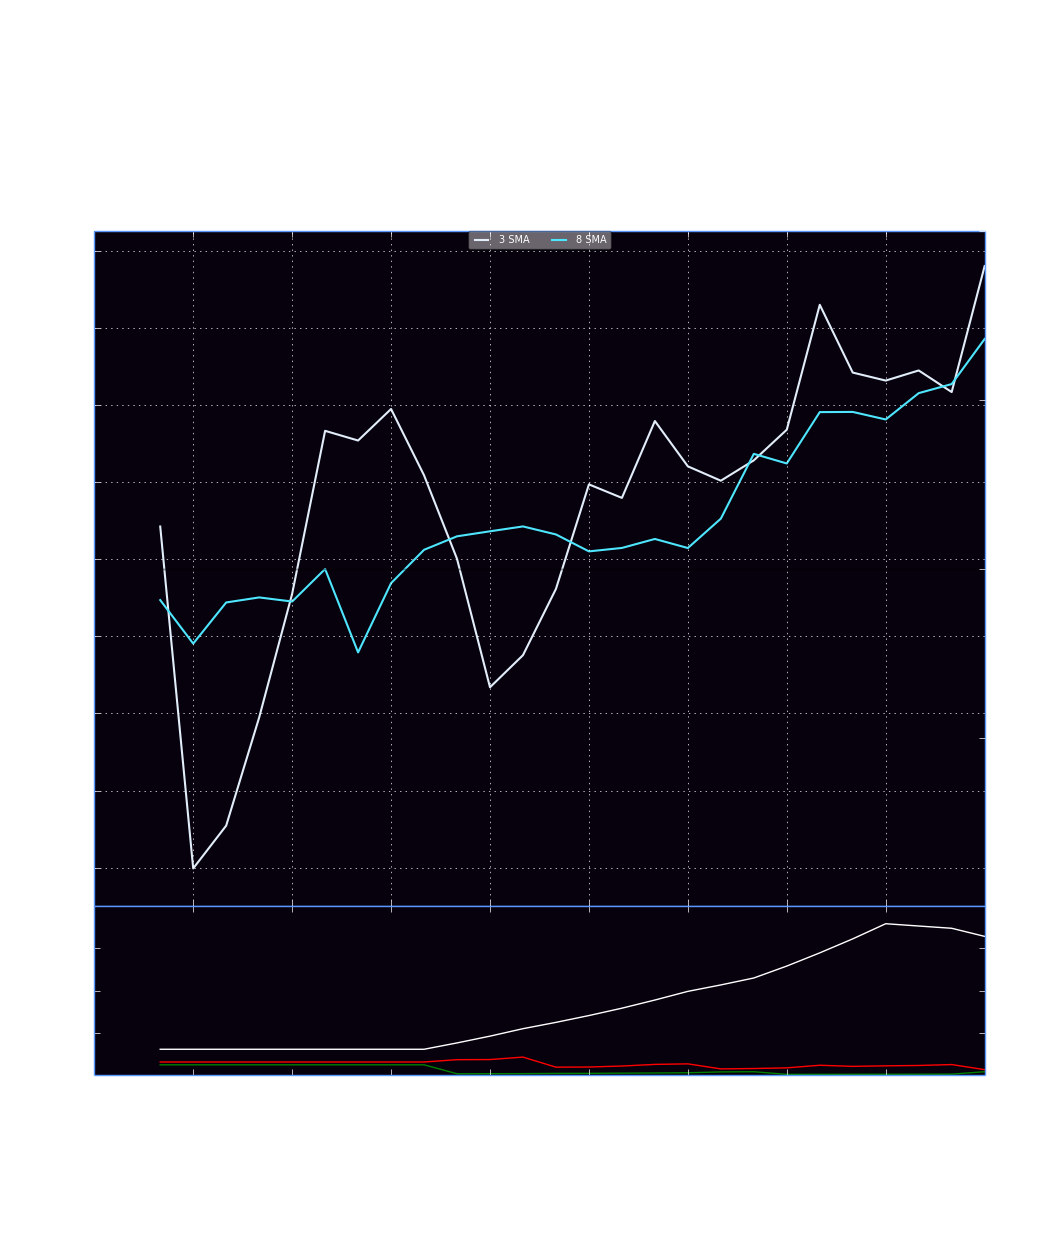
\includegraphics[width=\textwidth]{tweet_trend_plot.png}
    \label{fig:trend_tweet_plot}
    \caption{Tweet trend plot}
The graph show the average change in tweet sentiment between two days, over a 23 day period. 
\end{figure}
% 

\section{Trending in Finance}\label{trend:trends_in_finance}
We looked at the change at Oslo stock exchange in the same period as the tweets
above(Apr 30 - May 16). For the days the stock exchange was closed we padded out
the dataset with the previous open day. So that Saturday and Sunday would have
the same values as Friday. This is mainly to make the coding and plotting of
the graph easier. 

To describe the calculation of the finance trend: we took the percentage of
change in closing value from yesterday and today. Then we scaled the graph by a
value of 100 to make the changes visible in the same plot as the tweet trend.
\begin{python}
# calculate percentage diff between this and the previous day.
diff = (closing_value_today - closing_value_yesterday) / (
    average_value_today_yesterday * 1.0)

# scaled to work with the tweet trend.
results.append(diff * 100)
\end{python}

Plotting the graph we got figure \ref{fig:trend_finance_plot}.
\begin{figure}[htb]
    \centering
    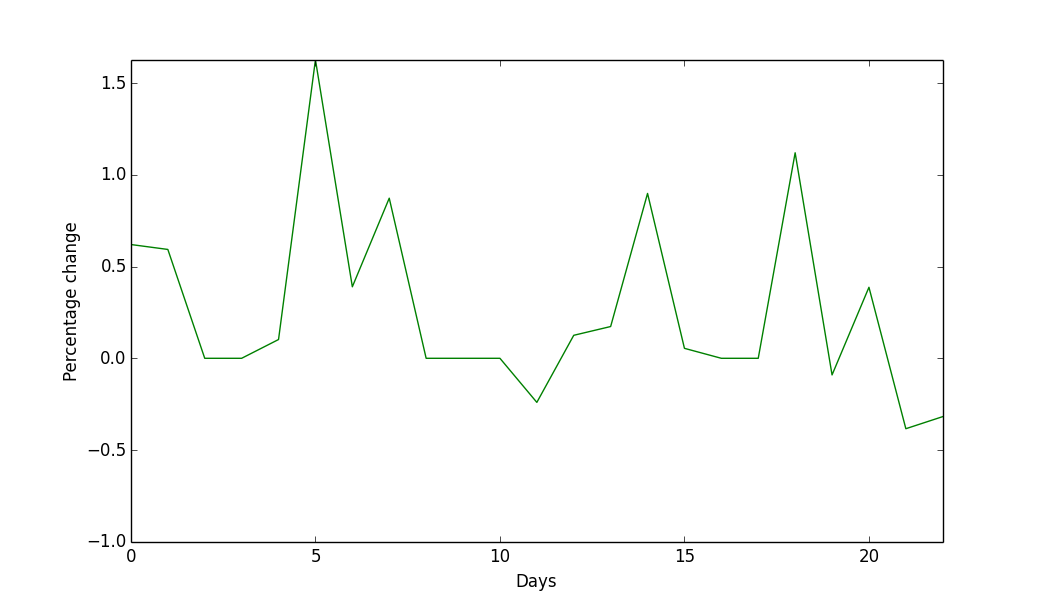
\includegraphics[width=\textwidth]{finance_trend_plot.png}
    \label{fig:trend_finance_plot}
    \caption{Finance trend plot}
The graph show the average change in closing value between two days, over a 23 day period. Note that the graph is scaled to be comparable with the tweet trend graph. 
\end{figure}
%

\section{Comparing the trends}\label{trend:compared}
First off, the trend plot in figure \ref{fig:trend_plot}. 
\begin{figure}[htb]
    \centering
    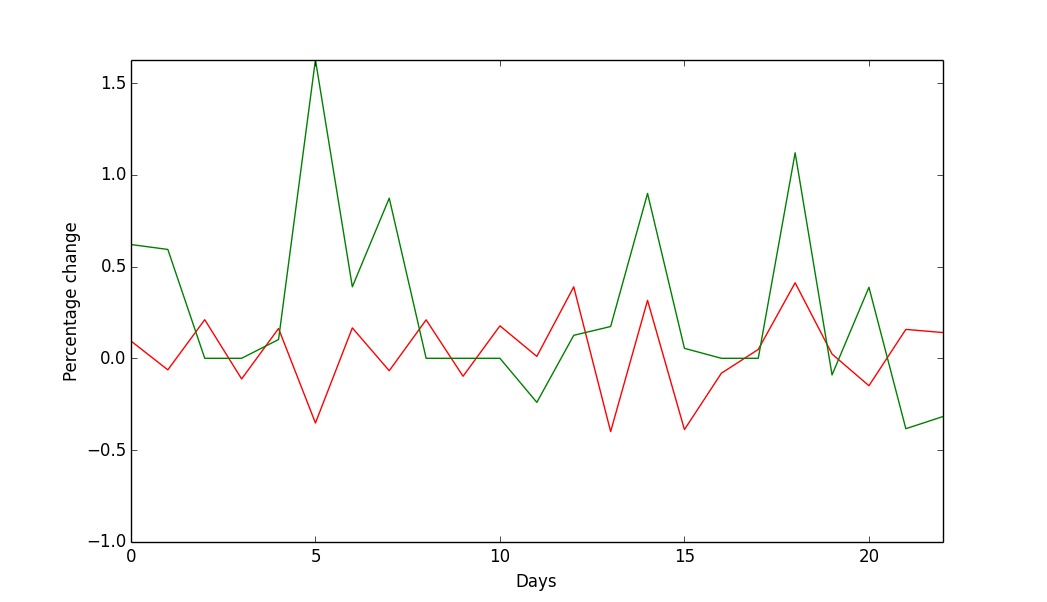
\includegraphics[width=\textwidth]{trend_plot.png}
    \label{fig:trend_plot}
    \caption{Comparing trend plot}
The graph shows the two previously compiled trends. The red one is the tweet
trend, while the green one is the finance trend.  
\end{figure}

And continuing with everything that is wrong with it. 

As correlations go between the two graphs we have very few. There are two areas
where the peaks are quite alike. At least the change is in the same directions.
This is at day 14 and 18. Besides those two points the graphs have no likeness
at all.  

What we can see from the plots is that the trend compilations have no
correlations. From this we can say for certain that the amount of data and way
of plotting the trends do not work.

The two things that are likely to play a big part in the results is the data we
used and the way we compiled the tweet trend. 

To narrow and to little data makes the result rather inconclusive. We should have
used something like a million of a billion tweets to get statistically
significant results.

And we should look closer on how we aggregate the twitter trend. Further we
should look at other fields of a tweet that can be significant for a trend. Like
followers and retweets.

From this we learn that data matters a lot and that it is difficult to find a
good way to aggregate a trend. 
%
